\chapter{Sharing a virtual world with people with dementia: A reflective account}
\label{NegotatingReseacherParticipantRelationships}

\section{Study one: Blending old with the new}
\label{StudyOne}
In November 2016, I started my final undergraduate year in the School of Computing at Newcastle University. Given my interests in  HCI and developing technology around dementia, the Head of School assigned my project to Dr Madeline Balaam and Dr Kellie Morrissey, who have similar interests in health and dementia. Given my family history with dementia, I was interested in exploring how technology could improve people's lives with dementia. My Grandpa was diagnosed with Alzheimer’s in his early 50’s, and my Grandma took care of him until he passed away when he was 67 (2001). I wanted to know more about the neurodegenerative condition and understand what my Grandpa and Grandma went through. 

At the time, virtual reality (VR) was gaining attention through the popularity of VR headsets and being picked up by the entertainment industry, particularly the gaming industry \citep{cipriani_understanding_2014}. When looking at the uses of VR for people with dementia, it was surprising to see a focus on neurological rehabilitation \citep{schultheis_application_2001,mendez2015virtual}. For instance, \citep{garcia2012discussion} proposed VR to offer brain-stimulating activities to reduce the progression of dementia. While this work is promising in their domains, at the time, prior work did not consider VR for people with dementia could function as an expressive and creative medium.

As such, by focusing on the growing body of work that has concentrated toward evoking emotion \citep{wallace_design-led_2013}, and creativity through technology with people living with dementia, this study aimed to consider how VR experiences for people with dementia might be sensitively designed to provide comfortable and enriching experiences. As I describe in the methodology, Sandra from Silverline Memories had also expressed interest in the design of Virtual reality on AppMovement where she describes the app as providing \textit{``images and scenes which could stimulate memory as well as providing comfort and reassurance to people with dementia or any memory loss''} (see figure \ref{fig:AppMovement-Sandra} for AppMovement quote). With Silverline Memories residing in the outskirts of Newcastle, my supervisors reached out to see if I could run a series of workshops at their dementia café as part of their afternoon tea sessions on Mondays. Dementia Cafés are places where people living with dementia, their families, and friends can come along and be part of a supportive environment that encourages opportunities for sharing experiences. These workshops had been organised to be flexible to co-exist alongside other organised activities within the dementia café. The aim was to get to know the members of Silverline Memories, and from getting to know one another, I could then curate a set of tailored VR experiences that would be interesting for the cafe.

\subsection{Workshop one: Getting to know the participants}
\label{StudyOne:W1}
\begin{figure}[htp]
\centering
\begin{subfigure}{.5\textwidth}
  \centering
  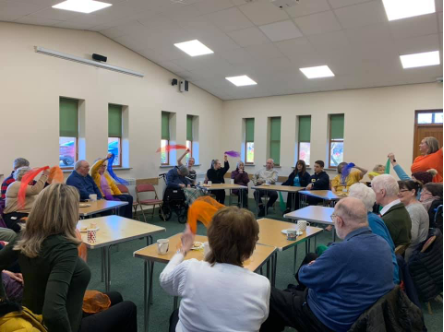
\includegraphics[width=.8\linewidth]{Images/ChapterFour/SilverlineCommunityRoomOne.png}
  \label{fig:communityRoomOne}
\end{subfigure}%
\begin{subfigure}{.5\textwidth}
  \centering
  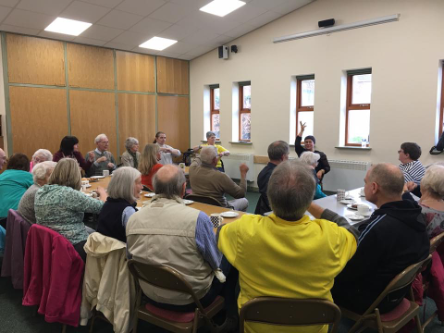
\includegraphics[width=.8\linewidth]{Images/ChapterFour/SilverlineMemoriesCommunityRoomTwo.png}
  \label{fig:communityRoomTwo}
\end{subfigure}
\caption{Silverline memories community room (taken from Silverline Memories Facebook)}
\label{fig:SilverlineCommunityRoom}
\end{figure}

For the first workshop, I wanted to find out what type of environments the members at Silverline Memories might want from a virtual reality experience. Working alongside Dr Kellie Morrissey, we set out to Silverline Memories dementia café, and I felt nervous. I felt so out of place. Apart from my experience with my Grandpa when I was a child, I had never really been around people living with dementia. Kellie and I arrived at the dementia café a little earlier than Sandra. Sandra came later than us with bags full of snacks and drinks for the members. As we approached the dementia café. We helped Sandra carry the bags into the the cafe (seen in fig \ref{fig:SilverlineCommunityRoom}). On the left side of the room was a kitchen area for volunteers to hand out tea, coffee and biscuits throughout the session, which had an open plan for volunteers and members to help themselves freely. 

Silverline memories had never had the chance to make space their own, with the community room being shared across many different groups. Instead, you had a sense of `home' or `community' emerging through the interactions with the volunteers and members. As I had set up the room, I got my notebook out, VR headset, a recorder, and consent/information sheets. As the first couple entered the café, Sandra and the other volunteers came over to them with open arms – similar to everyone who walked in on that day. They caught up, got them a cuppa tea and biscuits, and sat down. Sandra introduced the couple, Philip and Kate, who seemed enthusiastic to talk to us. They asked about the research, and what we did. However, as I would find out later on, the initial few minutes of signing consent, reading information sheets, and explaining the research are uncomfortable for all those involved. At that moment, it went from an informal conversation into a formal study where two of us would be analysing and studying what was said. As we described the study, both were very happy to participate in the conversation about the types of VR experiences they would like to see. They were okay with quotes being used as long as they were anonymised.

With VR being relatively new to the members, I began by introducing a simple VR experience which consisted of being placed in a virtual apartment as participants tried on a Google Cardboard headset. The decision for an apartment VR experience was decided for its neutral nature; it did not give any low or high expectations for what to expect with VR technology. After participants tried the headset, we spoke about the type of places they would like to see through the VR headset. I used printouts of images to further these conversations, such as images of libraries, museums, forests, and beaches. During the first workshop, I spoke for an extended time with one couple, Thomas and Janet, where Janet was living with dementia. The couple told me about Janet's preferences for a VR environment that emphasised country music. From this, I decided to create a personalised VR experience based on her love for Shania Twain. I also set out to design and develop environments for the dementia café. The first was a beach environment, and the second was a park that took inspiration from a local park that participants had reminisced about in the workshop. Thirdly, as briefly mentioned above, I sought to design a bespoke Shania Twain concert hall experience for Thomas and Janet.

The workshop was my first experience working with people with dementia, but more importantly, the first time I would be seen as a' researcher'. Although I looked young and got sarcastic comments from the participants about my age, I did not know how to conduct myself in conversations with this new title. Each conversation felt like an interview, and I sensed a power imbalance. In some instances, power imbalance came from both sides, with members of Silverline Memories having been a part of the café for some time. Members did not have to talk to us or participate in the study, and if they did not, they had nothing to lose.

On the other hand, Kellie and I were the only ones walking around with the title of' researcher' who were here to interview and record participants. It was so unnatural to me, but why would it be natural? I do not start my conversations with friends or family with consent forms and placing an audio recorder on the table. Nevertheless, the methodologies I was told to follow focused on the importance of researcher-participant relationships. For instance, \cite{mckillop2004make} highlight the importance of building relationships with people with dementia to make participants feel more comfortable in the study. The authors provide several strategies to improve engagement in interviews, such as talking about the person's life and what they have done today; being empathetic and caring in the interviews; and being flexible in the conversation to fit the participant's needs.

\subsection{Designing Tailored VR environments}
\label{S1:VREnvrionments}

\begin{figure}
\centering
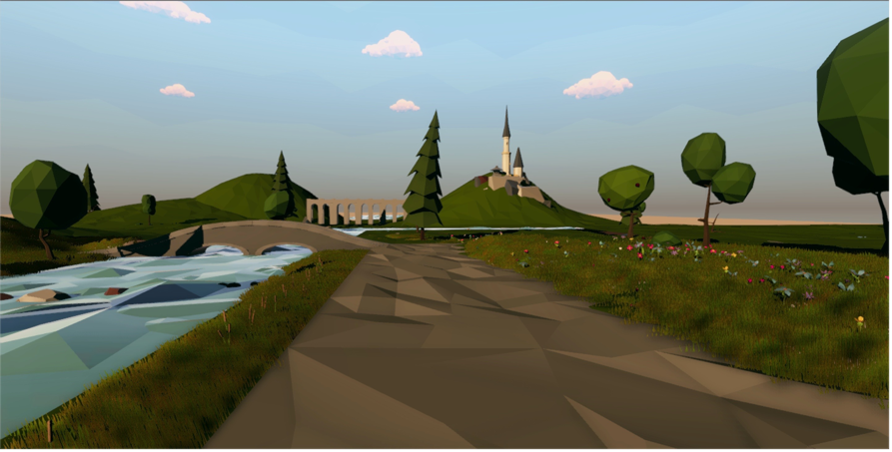
\includegraphics[width=.8\linewidth]{Images/ChapterFour/IrishCastlVR.png}
\caption{Park environment including an Irish castle}
\label{fig:IrishCastle}
\end{figure}

From the data collected from our first workshop, I created sketches based on individuals' ideas and desires. While I could not develop each participant's individual experience due to time constraints, some ideas were combined into one environment. For example, from my field notes, one participant asked to \textit{`take [her] back to Ireland, to see the beautiful castles again’}. While I could not do that, I did create 3D designs of a traditional castle from Irish medieval architecture. We placed it in the park environment that many participants expressed interest in (see Fig.\ref{fig:IrishCastle}).

I created all three VR environments in the Unity game engine. I carefully planned the design of our environments in terms of the participant's field of view. I applied \cite{alger_visual_2015} concept of content zones described in Fig.\ref{fig:ContentZone} to reduce risks of sickness or disorientation and to improve the overall experience for the individuals. At the time, designing realistic VR experiences was limited to using 360-degree cameras. As I wanted to create experiences that may not be available, such as a 360-degree Shania Twain concert, the design of the environment was based on low-poly art that not only can run on low-end hardware (a simple smartphone) but which also provides a very stylised and abstract view of the reality.

\begin{figure}[htp]
\centering
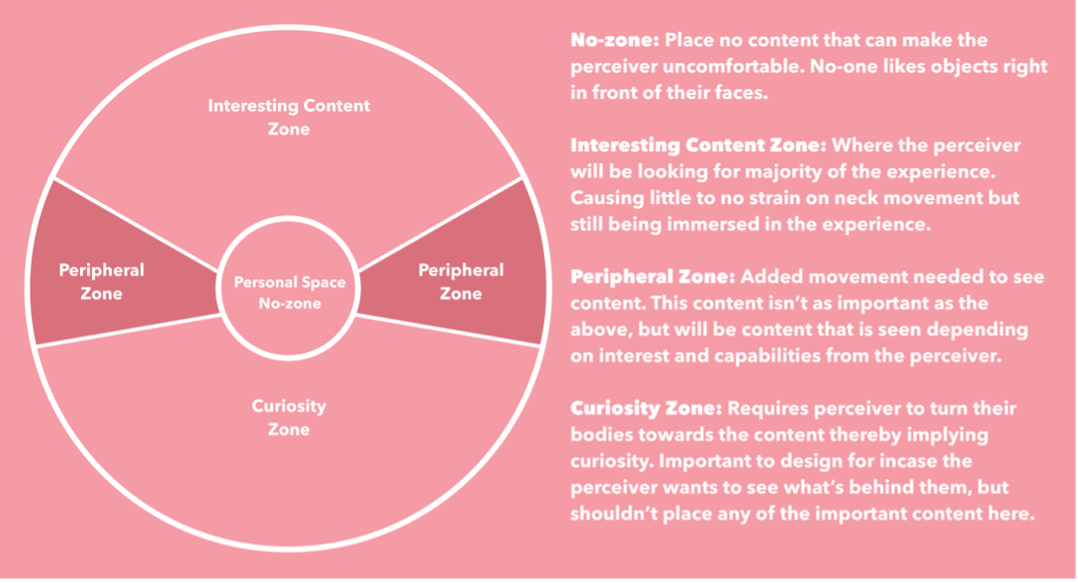
\includegraphics[width=.8\linewidth]{Images/ChapterFour/ContentZones.png}
\caption{Content zones in VR}
\label{fig:ContentZone}
\end{figure}

\subsection{Workshop two: ``Lighthouse, Rocks, Sand, Sea, Boat!''}
\label{StudyOne:WorkshopTwo}
In the second workshop, I returned to Silverline Memories to try out the different environments focused on the group at large: the beach with a horse running along the sand and a park based on a local park nearby, Jesmond Dene. Given that the charity had recently won a lottery fund, the volunteers provided celebration activities such as a magician and a singer. The celebrations put less pressure on me, as the entertainers kept the room occupied while I gradually went around the room and showed the VR environments to attendees. 

Multiple care partners and people with dementia tried the park and beach experiences and adored them. With encouragement from her daughter, Lucy, living with dementia, tried the beach experience and started listing what she could see — \textit{``lighthouse, rocks, sand, sea, boat!''} — as she rotated around and took control of the experience by focusing on the parts of the environment she found interesting. In this instance, Lucy was not a passive observer in the experience, but in fact, the focal point driving the experience. Lucy continued to talk about the experience to her daughter, which added to a shared experience for the two. In this way, the technology acted as a novel experience that provided an excuse or conduit for conversation - similar to `ticket to talk'. \cite{welsh_ticket_2018} discusses, in their design of Ticket to Talk, an app to provide conversational guidance in dementia, that carefully designed technology can provide essential conduits for a social chat in dementia when social partners are unsure what to talk about. By tailoring the VR environments to the participant's interests, often, participants would comment on identifiable objects or reference memories associated with the beach or the park.

They are not the only couple who found the opportunity to share meaningful experiences. Many, if not all participants, expressed a wish to be able to share in the same live VR experience as their partner or parent. When asked about this, participants indicated that meaningful shared experiences with their loved ones with dementia had changed recently or decreased in frequency. For example, Linda, whose husband Michael is living with dementia, mentioned that the couple no longer drive and had to use public transport. This meant that the two could not visit favoured locations together, and so indicated that the VR park and beach could be used to supplement their recreational activities and allow them to experience a semblance of the sorts of activities that used to mean very much to them. Having the carers experience the environment first allowed carers to help direct their loved ones around the environment by being able to probe specific interactions in the environment that the person living with dementia may have missed. For instance, one carer started asking questions about what they could see or if they saw the horse walk past on the beach. 

In addition to this kind of shared experience would be an external screen that displays the same view as the headset. Recently, with the increased interest of Facebook on VR headsets, with the Oculus series, being able to stream your headsets display to your phone is significantly more accessible than it was in 2017. A suggested interaction toward VR shared experiences would be for carers to be able to interact with the VR environments through their external display alongside the person living with dementia driving the experience from the VR headset. However, when designing aspects of training or testing into VR environments, they should be separate from those environments that aim to be recreational. To implement aspects of training or testing into these environments would mean returning to a medicalised view of the person with dementia as a set of deficits, rather than a fully realised person with needs and desires \citep{lazar_critical_2017}.

Near the end of the workshop, I sat down with Thomas and Janet to show them their personalised Shania Twain concert hall. With the current room getting quite loud, we asked the couple to sit down in the back room at the dementia café as a significant part of the experience was linked to the music itself. As I set the VR headset and passed it over to Janet, Thomas expressed some initial concerns about Janet having ‘the patience to hold the [headset] for a long time’. Thomas initially aided her in holding the VR headset:

\begin{quote}
\textit{Straight away [Janet] started to sing. She was singing to the tune and attempted to repeat the lyrics… [and] changed her body language completely. It went from rather static, to movements that captured the tempo of the music. Janet held up her hands to try to hold the Google Cardboard as well, which indicated she did not want to stop the experience. [Afterwards], she seemed very happy and just from being around her, you could see her mood had changed completely.}    
\end{quote}

While Janet’s experience was heightened by her ability to recall the Shania Twain song, she got to experience it in a completely new way. While her verbal abilities are limited, other means of communicating became apparent. Janet’s interests, body movement, and overall socialness in the café significantly changed after experiencing the concert hall. The bespoke design that placed Janet at the forefront of the design, and who could drive the experience, has a freeing effect that is pleasurable for participants who can engage in enjoying activities; lately, reflecting on the experience, Thomas mentions that Janet has \textit{``always sang and whistled. She can sing along to songs as long as she remembers the words. The aesthetic of the theatre was a great idea and gave a great sense of space''}.

\subsection{Reflections and outcomes}
\label{S1:ReflectionsOutcomes}
I embarked on this study with interest in learning more about dementia that I have family ties with. During the conducting of the study described above, I was able to have multiple conversations about dementia with my Grandma and understand her relationship with dementia. Through these conversations, I was able to connect to my Grandpa, who I never thought I would have the chance to. Listening to my Grandma's stories of looking after my Grandpa painted a picture of a relationship with 'ups and downs', with an overall positive perspective of dementia. However, only by spending more time at Silverline Memories did I gain a more in-depth understanding of the vastly different experiences people have with dementia. To conclude this section, I reflect on the following four areas:
\begin{enumerate}
    \item Feeling foolish in VR.
    \item Designing for reminiscence.
    \item The robustness of the technology.
    \item To what extent is this co-design?
\end{enumerate}

\subsubsection{Feeling foolish in VR}
\label{S1:Foolish}
From the initial workshops, my research into VR has continued to bring up themes and conversations around feeling isolated or the fear of looking silly. This tendency of feeling silly in VR is relatively standard among many who have tried VR. While this is not focused purely on dementia, a diagnosis of dementia can heighten these feelings as dementia progresses. \cite{nolan_perceptions_2006} reported examples of people living with dementia feeling embarrassment and shame if others became aware of their dementia. Nolan expands further that stigma and embarrassment become apparent in fear of people witnessing \textit{``inappropriate behavior in public''}. With VR being isolating and looking silly, it is not surprising that I had participants feeling uncertain about taking part in activities, as a way to protect their dignity. Beyond the remarks about VR headsets looking silly, participants expressed concerns about comfortability and weight that I describe in detail in a CHI'18 paper - \citep{hodge_exploring_2018}. In this study, I used a Google Cardboard headset which is not comfortable, but many preferred to use this as it was lightweight and was comfortable to hold. Over the last few years, we have seen massive strides toward comfortable and attractive headsets, especially ones that do not require wires that connect to a computer. However, they remain moderately on the heavier side, and while attractive, they can tend to look remarkably futuristic and off-putting. Future designs could benefit from thinking about how headsets could fit into spaces and look normal — e.g., by embedding the display into a set of binoculars or a spectacle with a handle.

\subsubsection{Designing for reminiscence}
\label{ReminiscencevsMoment}
During the first workshop, participants expressed particular locations that resonated with their childhood. For example, several participants who grew up in Newcastle described seeing Jesmond Dene Park or Whitley Bay Beach - with both places being popular days out' places in the North East. During the converastions, participants would often describe structural details such as \textit{``I love the bridges over the lake''}, and stories of Whitley Bay lighthouse. Those not from Newcastle expressed other childhood memories and locations, such as one participant asking to \textit{``take [her] back to Ireland, to see the beautiful castles again''}. Drawing on childhood memories mirrors the use of technology to support the collection of media such as photos, texts, or other memorable artefacts, from the person with dementia's past. The media can then be used for conversation, reminiscence, and interaction between the person with dementia and family care partners and care staff. As such, one of the key insights in this work was the wish for shared experiences and the potential for VR experiences to promote conversation. 

While prior work, including my own, has leveraged techniques such as reminiscence, I believe in some instances that this can limit the active participation of the person living with dementia in these design processes. While reminiscence can provide opportunities for engagement \citep{gowans_designing_2004, yasuda_effectiveness_2009}, for some, it may merely be non-engaging or cause frustration when not being able to remember a specific memory from their past \citep{lazar_using_2014}. Further, centring an activity around the stability of long-term memory can lead to distress and raised expectations for the person with dementia who may not connect with the activity meaningfully. While Janet had a clear connection with Shania Twain, which supported the overall enjoyment of the experience, the experience might have been disinteresting or frustrating to both Janet and Thomas if Janet had not recognised the music. In contrast, other work that aims to provide a failure-free environment has been exemplified by systems such as CIRCA \citep{alm_communication_2007}. The CIRCA technology consists of a touch screen that displays music, video, photos and text to support general reminiscence rather than targetting specific life experiences or relationships.

Therefore, we must question whether approaches that rely on the person’s ability to recognise or articulate past events are an appropriate activity to enhance emotional connection. Similarly, we might also ask how we could provide opportunities for people to interact with evocative immersive experiences with differing emotional valence. It could be that they are not necessarily ‘pleasant’ memories, but are not distressing, and are valid and important experiences with which it may be valuable to interact.

\subsubsection{The robustness of the technology}
\label{S1:Robustness}
With the study being exploratory work that would consist of two workshops, there was not enough time to develop a robust product that could stay with Silverline Memories. At the time, I knew that the three environments I made were very rough prototypes that were prone to breaking and very limited to working on my phone device. Knowing the condition these prototypes were in, I never thought they would be ready to be deployed and used without my assistance to set up and solve unexpected software crashes. \cite{hwang2020exploring} further discourage leaving technology that might be in the prototype stages. If the technology evokes "frustration, anxiety or sense of vulnerability", the person with dementia might resist the technology altogether. This resonates with \cite{vines_our_2017}, who describes participants' frustrations with using Google Glass, which stopped supporting the product resulting in an outdated product with bugs typically found in prototypes. 

Additionally, \cite{hwang2020exploring} stresses the importance of care partners' and volunteers' training, configuring and supporting the person with dementia in using technology. Similarly, in this study, care partners demonstrated this role in encouraging the use of virtual reality and asking questions about what the participant could see in the virtual environment. In this way, the leaving of technology requires more robust working products and upskill care partners or volunteers to know how to use the technology and support the learning process of accessing the VR environments. 

\subsubsection{To what extent is this co-design?}
\label{WhatExtentCo-design}
As described in the background literature and methodology, several researchers have innovated many of the methodological approaches to support people living with dementia to engage meaningfully in the design and development of technology. For this study, although I did not have sufficient time with the participants to effect a truly co-designed process, I spent more time with Thomas and Janet to inform the building of the Shania Twain concert hall. In part, this was opportunistic from Sandra expressing interest on behalf of Thomas, who could see the potential value of VR for people with dementia. During the first workshop, Thomas and I talked at length about the potential of VR and how Janet may use it. This led to talking about Janet's favourite songs and how he curates Youtube playlists at home. By the end of the conversation, I had expressed interest to Thomas in building a concert hall around Janet's favourite musical experiences.

While we had generated an idea together for the VR environment based on Janet's interests, that was the extent to which people with dementia were involved in the pre-design process. In workshop two, people with dementia were involved in the evaluative stages to understand how people with dementia might use VR and the potential issues with current VR technology. Rather than the work being co-design, the process was more towards a consultation of the types of interesting experiences people with dementia might need. Further, given Janet would rarely speak, Thomas spoke on her behalf and indicated the type of interests she might want. While this worked well in this instance, this raises several questions: To what extent can people with dementia contribute to the pre-design phases? If so, are people with dementia acting as an equal part in the discussion, or rather, engaging in a set of workshop activities that provide the opportunity to co-create? \citep{tsekleves2020engaging}

\section{Study two: Media capture of meaningful experiences}
\label{studyTwo}
Motivated by the outcomes of the previous study, the following study explored the role of rich, personalised media experiences as a support for families with dementia. Taking account of the ecology of care of the person with dementia, which considers the person with dementia, friends, and family, the experiences I created in this study needed to be meaningful to the family — not just the person living with dementia. In response to the reflections above, this study set out to tackle the reflections by:

\begin{itemize}
    \item \textbf{Feeling Silly in VR}: To respond to the discomfort around wearing and navigating VR, this study designs multiple ways to experience VR environments, from bespoke VR tour guides, to scanning QR codes to exploring 360-videos on a tablet or phone. 
    
    \item \textbf{Designing for reminiscence}: Instead of relying on the person's abilities to recognise or articulate past events, this study orients experiences towards being in the moment and living a meaningful life with dementia.

    \item \textbf{Robustness of technology}: While this study focuses on building prototypes to explore the ways technology might be used by people with dementia, an output of this work was for the families to be provided with a VR headset and additional materials made post the end of the study.

    \item \textbf{To what extent is this co-design?}: In the first study, participants had little input on what would be created for the VR environments. This was primarily due to the short turnaround of the project. For this project, I worked with the families over numerous visits and co-designed days out to leverage the walking interview technique described in the methodology.
\end{itemize}

Working with Silverline Memories again, I carried out a Research Through Design (RTD) methodology. RTD is a way of doing research which is the practice of design used to address wicked problems [56], which entail a sense of complexity, and which have no cur- rent solution. RTD seeks to address the problem within its current situation and is generally acknowledged to involve end users within the design process in order to result in the addressing of, and reflecting on, problems within the associated design space. The output of RTD is the creation of artefacts, digitally-mediated experiences, and systems, which are applied to new problems to create new knowledge [5, 19, 70]. The knowledge produced can only be elicited by the creation of these artefacts, which offer a novel and embodied method of knowledge production. The study aimed to explore the opportunities and challenges of designing personalised multimedia experiences with people living with dementia and their families. As stated above, the previous study focused on the concept of reminiscence, with myself developing the VR environments after the workshops. For the second study, considering how I might capture experiences of being in the moment, I aimed for the families to capture themselves using 360-degree cameras. I worked with three families: two married couples, both with a wife living with dementia, and where the husbands had formed a close relationship through attending a support group. The third family was a family of four, where the father was living with dementia. 

To begin conversations with families about participating in the project, I met the families at one of the Silverline Memories days out. I used this as an opportunity to get to know the families, explain the research and purpose. Sandra introduced the two married couples (Lauren, Michael, Sarah and John), who seemed somewhat sceptical of participating. Initially, Michael jokingly would ask if I would be \textit{``spying on them''}, or how I \textit{``look awfully young to be a researcher''}. These jokes distinctly made me stand out from the rest of the group. There was a clear divide between who I was and their community. At the time, I felt like I had to prove that I was invested in what they had to say, and I was not here just to collect data and then leave. 

Similar to the reflective piece in the methodology, Michael asked \textit{``why are you so interested in us?''} I told Michael stories about my Grandparent's relationship and how I wanted to know how technology could improve the quality of life for families with dementia. This led to Michael  opening up about the importance of relationships and friendship when Lauren was diagnosed with dementia:

\begin{quote}
\textit{``It's been a few years since Lauren was diagnosed with dementia, and Silverline Memories has been a lifeline for us. At first, I didn't know what to really do... We would just sit inside all day and Lauren would just look at the wall and not do anything. But then a friend of mine started to tell me to start going to these dementia activity days like Silverline, and that is where I met John and Sarah. Since then, it has been life-changing. We go on holidays, spend most of our weekdays together, and try to do as much as possible.''
}    
\end{quote}

It was apparent how meaningful the relationship was between Lauren, Michael, Sarah and John. From Sarah and Lauren's diagnosis, the four of them depended on one another, not just for enjoyment, but for Michael and John to depend on one another for support. As we continued to talk and spent the day getting to know the couples, Michael and John both ended up being very keen on taking part in the research. I sat down with the four of them, and we planned out a day out at a National Trust park in Northumberland. I took their phone numbers, and we scheduled the rest of the day out over the phone.

\subsection{Day out with `The Fabulous Four'}
\label{DayOutOne}
For the first day out, I went out on a day out with John, Sarah, Lauren and Michael - also known at Silverline Memories as 'The Fabulous Four'. The families decided on the National Trust Site in Northumberland as this was a place that Michael and Lauren had become fond of over the past decade. As travelling can cause discomfort to many, I hired the driver (Dave) from Silverline Memories, who not only gave comfort to the families as he was a familiar face, he acted as a tour guide, which the families appreciated and found his presence to be enjoyable. The family directed our day to capture moments they would like to experience again through personalised media. I captured these moments using photography, audio-recordings, as well as more contemporary technologies such as 360-degree video cameras. On the day out, I spent time with the family as more than just an observer. I took part in activities set out by the families, engaged in conversations and helped with capturing specific moments the families wanted throughout the day. The day out captured insights into each family’s history, the families’ care for the person with dementia, and meaningful interactions between the family members.

When conducting the first two workshops in the first study, there was a lack of design decisions being made by people with dementia. A significant portion of the conversations I had seemed to be with their care partners, where they would speak on their spouse's behalf. However, when engaging with the VR headsets, people with dementia were active participants rather than passive. As such, the potential for using 'day out' or 'walking interviews' (that I describe in methodology chapter section \ref{PD:Interviews}), could potentially make the person with dementia feel at ease, self-regulate their talk and, in their own time, share their experiences through their abilities.

The procedure started by sitting down at Michael's and Lauren's home, where the group suggested we meet. The pre-day-out conversation was relatively straightforward, reiterating the study and filling out consent forms. Once consent was filled in, Dave, the driver, drove the group to Wallington National Trust. Once at the site, I encouraged the family to decide where to walk through the day, including when they wanted to return home and if they wanted to sit down and have lunch or a rest. For capturing 360-degree videos and photography, the family would direct me around the day. For instance, John would suggest \textit{``Hey, can we go to the Chinese Pond and you could capture some videos of us walking through the place?''} The interview process had an open-ended style and had the characteristics of a conversation rather than an interview. During the day, I would often lead the conversations by following up on the participant's comments about the day, or reacting to their nonverbal (i.e. picking up some bark on the floor through the forest).

\subsection{The families active role in the day out}
\label{ActiveRole}
Throughout the day out, interactions with the family seemed radically different from previous conversations. Having a continuous activity seemed to stimulate sharing of knowledge between everyone involved. This section introduces three interactions with the couples, which shaped my understanding of walking interviews and allowed me to get to know the families.


\subsubsection{Taking lead}








 Lauren taking lead

\begin{quote}
\textit{   \textbf{Lauren}: ``You take note because I forget which way I come from, where I'm going to.''
}\end{quote}

\begin{quote}    
\textit{    \textbf{Researcher}: ``Don't worry. No problem. If we get lost, we'll get lost together. That's fine. It's so beautiful. You've been here quite a few times. Is that right?''
}    \end{quote}
    \begin{quote}    

\textit{    \textbf{Lauren}: ``Yes. Yes.''
}\end{quote}




Michael - stories - sat down
We ended up in a little village called Farnworth. And in Farnworth there's a stream that runs through it. There is a road bridge, and underneath the road bridge, there is a deep place where you can get your horse in and you can wash all its legs off and get all of the mud off the bottom of it. Then . . . [a lady] went right under, which of course was hilarious to some of us who were still slightly uninhibited. But I can see the whole thing in my mind. It was just a fun day. It's all down to 150% whiskey spirit.

Diromas toys

Sarah: Oh wow, look at how lovely these are! *pointing at the minitaure figurine set*

James:  Imagine having one of these to play with when you were younger

Sarah: Oh I know. It is incredible! Look at these little ones here *prompting me and Lauren to have a look*

Lauren: Ah they're lovely aren't they

Keith: You had something like that when younger Sarah didn't you?

Sarah: Absolutely. its fantastic

Sarah and lauren continued to grab my attention to the fine details of the different minitaure furniture.


telling me about how much they use to love to play with them and would love to do it again



Summary 
therapy -- happy after walking interview








